\FloatBarrier
\subsection{Database e mapping}

L'applicazione usa come supporto un database relazionale contenente i dati rigurdanti le aule dei vari edifici universitari e del personale.
\`E fondamentale però mettere in evidenza con un adeguato schema Entità/Relazione le tabelle utilizzate all’interno del progetto e create al fine del corretto funzionamento del 
sistema.

\begin{figure}[!htb]
\centering
\includegraphics[scale=0.60]{databaseER.png}
\caption{Diagramma E/R del database}\label{fig:database}
\end{figure}

Facendo riferimento alla figura \ref{fig:database}, descriviamo le entità fondamentali definite nel modello in esame:
\FloatBarrier
\begin{description}
\item[Room]\`e l'entit\`a principale. Essa contiene le informazioni riguardanti una specifica stanza di un determinato piano di un edificio. 
\item[Building]rappresenta l'edificio, caratterizzato da un numero univoco e dotato di un nome.
\item[Person]rappresenta il personale. Fondamentale per l'applicazione sono il ruolo di una persona (ad esempio docente e ricercatore) e le date di fine e inizio contratto lavorativo.
\item[OccupyRoom]associa una persona a una o pi\`u stanze diverse e  servir\`a ad ottenere una lista delle persone che occupano una stanza.
\end{description}

\FloatBarrier
\begin{figure}[!htb]
\centering
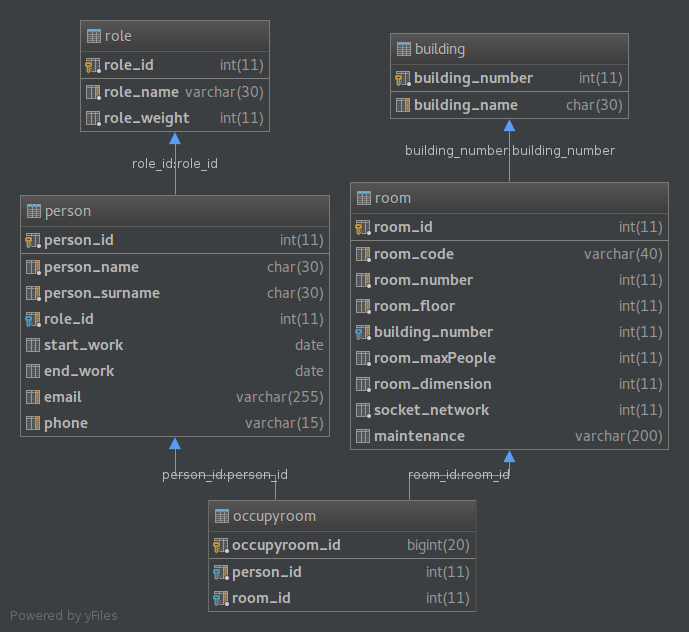
\includegraphics[scale=0.55]{diagram.png}
\caption{Modello Relazionale del database}\label{fig:databaseRelaz}
\end{figure}
\FloatBarrier
Dopo aver sviluppato il modello relazionale(figura \ref{fig:databaseRelaz}), tramite una metodologia bottom up, sono stati interfacciati oggetti Java con il database relazionale attraverso file di mappatura XML, uno per ogni classe che si vuole rendere persistente.\\ 

\begin{figure}[!htb]
\centering
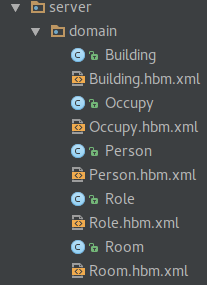
\includegraphics[scale=0.55]{packageMapping.png}
\caption{Package contenente i file di mappatura e le corrispondenti classi Java.}\label{fig:mappingPack}
\end{figure}
\FloatBarrier
Questi file di mappatura sono caratterizzati  dalle dualità classe-tabella e attributo-colonna.
Per inviare le informazioni al client non si possono sfruttare queste classi utilizzate per Hibernate. Infatti, nonostante implementino Serializable, vengono interpretate in modo particolare dal compilatore (la libreria Javassist si occupa di riscrivere il bytecode di tali oggetti Hibernate) e quindi, quando devono essere serializzate o deserializzate per essere trasmesse al client, il meccanismo GWT RPC non sa come trattarle e le rifiuta. Per risolvere questo problema si fa uso di classi DTO (Data Transfer Object). Le classi DTO sono delle semplici classi contenenti esclusivamente i dati che si vogliono memorizzare senza la logica per la persistenza aggiunta da Hibernate; queste sono quindisfruttabili a lato client e utilizzate poi per "costruire" le classi Hibernate.
\begin{figure}[!htb]
\centering
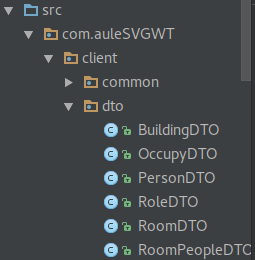
\includegraphics[scale=0.45]{dtoScreen.png}
\caption{Classi DTO}\label{fig:dtoPack}
\end{figure}